% !TEX root = master_thesis.tex
\chapter{Event selection}
The determination of polarization observables needs to be completed for particular reactions (cf. chapter \ref{chap:intro}), such as the photoproduction of e.g. a single $\eta'$ meson. However, the recorded events  contain data from the decay products of all possible final states in addition to combinatorical background. Thus, event candidates for the desired reaction have to be extracted before they are considered for further analysis. Table \ref{tab:etap} shows the five most probable decay modes of the $\eta'$ meson. Three of these result in final states which only contain photons and are thus accessible for reliable measuring with the CBELSA/TAPS experiment. Only the $\eta'\to\gamma\gamma$ decay channel was considered for further analysis; the $\omega\gamma$ channel provides negligible statistics and considering the acceptance of detecting six photons in the final state, the expected yield of the $\eta'\to\gamma\gamma$ decays should be roughly equal to the $\eta'\to\pi^0\pi^0\eta\to6\gamma$ final state \cite{farah}. Offering a cleaner, three-particle final state, the $\eta'\to\gamma\gamma$ was then favored in the course of this thesis.      
\begin{table}[htbp]
	\centering
	\begin{tabular}{clc}
		\toprule
		\multicolumn{2}{c}{Decay mode}&Branching ratio\\
		\hline
		$\pi^+\pi^-\eta$&&42.6\%\\
		$\rho^0\gamma$&$\to\pi^+\pi^-\gamma$ &28.9\% (28.9\%)\\
	$\pi^0\pi^0\eta$&$\to6\gamma$ & 22.8\% (8.8\%)\\
		$\omega\gamma$ &$\to (\pi^+\pi^-\pi^0\gamma/\pi^0\gamma\gamma)$&2.52\% (2.2\%/0.21\%)\\
	$\gamma\gamma$&&2.3\%\\

		\bottomrule
	\end{tabular}
\caption{The five most probable decay modes of the $\eta'$ meson. The most probable further decay with according branching ratio is shown in brackets.\cite{pdg}}
\label{tab:etap}
\end{table}
The process of \emph{event selection} for the reaction $\gamma p \to p\eta'\to p\gamma\gamma$ is outlined in the following chapter.

\section{Charge cut}

\section{Time of particles}
Due to its high count rate the tagging system (see section \ref{subsec:tag}) will not only record beam photons which produce the detectable final state particles, but also several uncorrelated beam photons. To select only beam photons which will induce a photoproduction process the time information of the detected particles is used. It is shown in figure \ref{fig:time} for all particles involved in 3PED events of $\eta'$ photoproduction. In all cases prompt peaks centered around \SI{0}{\nano\s} (the trigger time) are visible. Since the final state photons move with velocity $c$ their timing information does not underlie fluctuations, as is the case for the final state proton on the contrary. The tagged, uncorrelated beam photons are visible as flat background underneath the prompt peak in the time of the beam photon.

\begin{figure}[htbp]
	\centering
	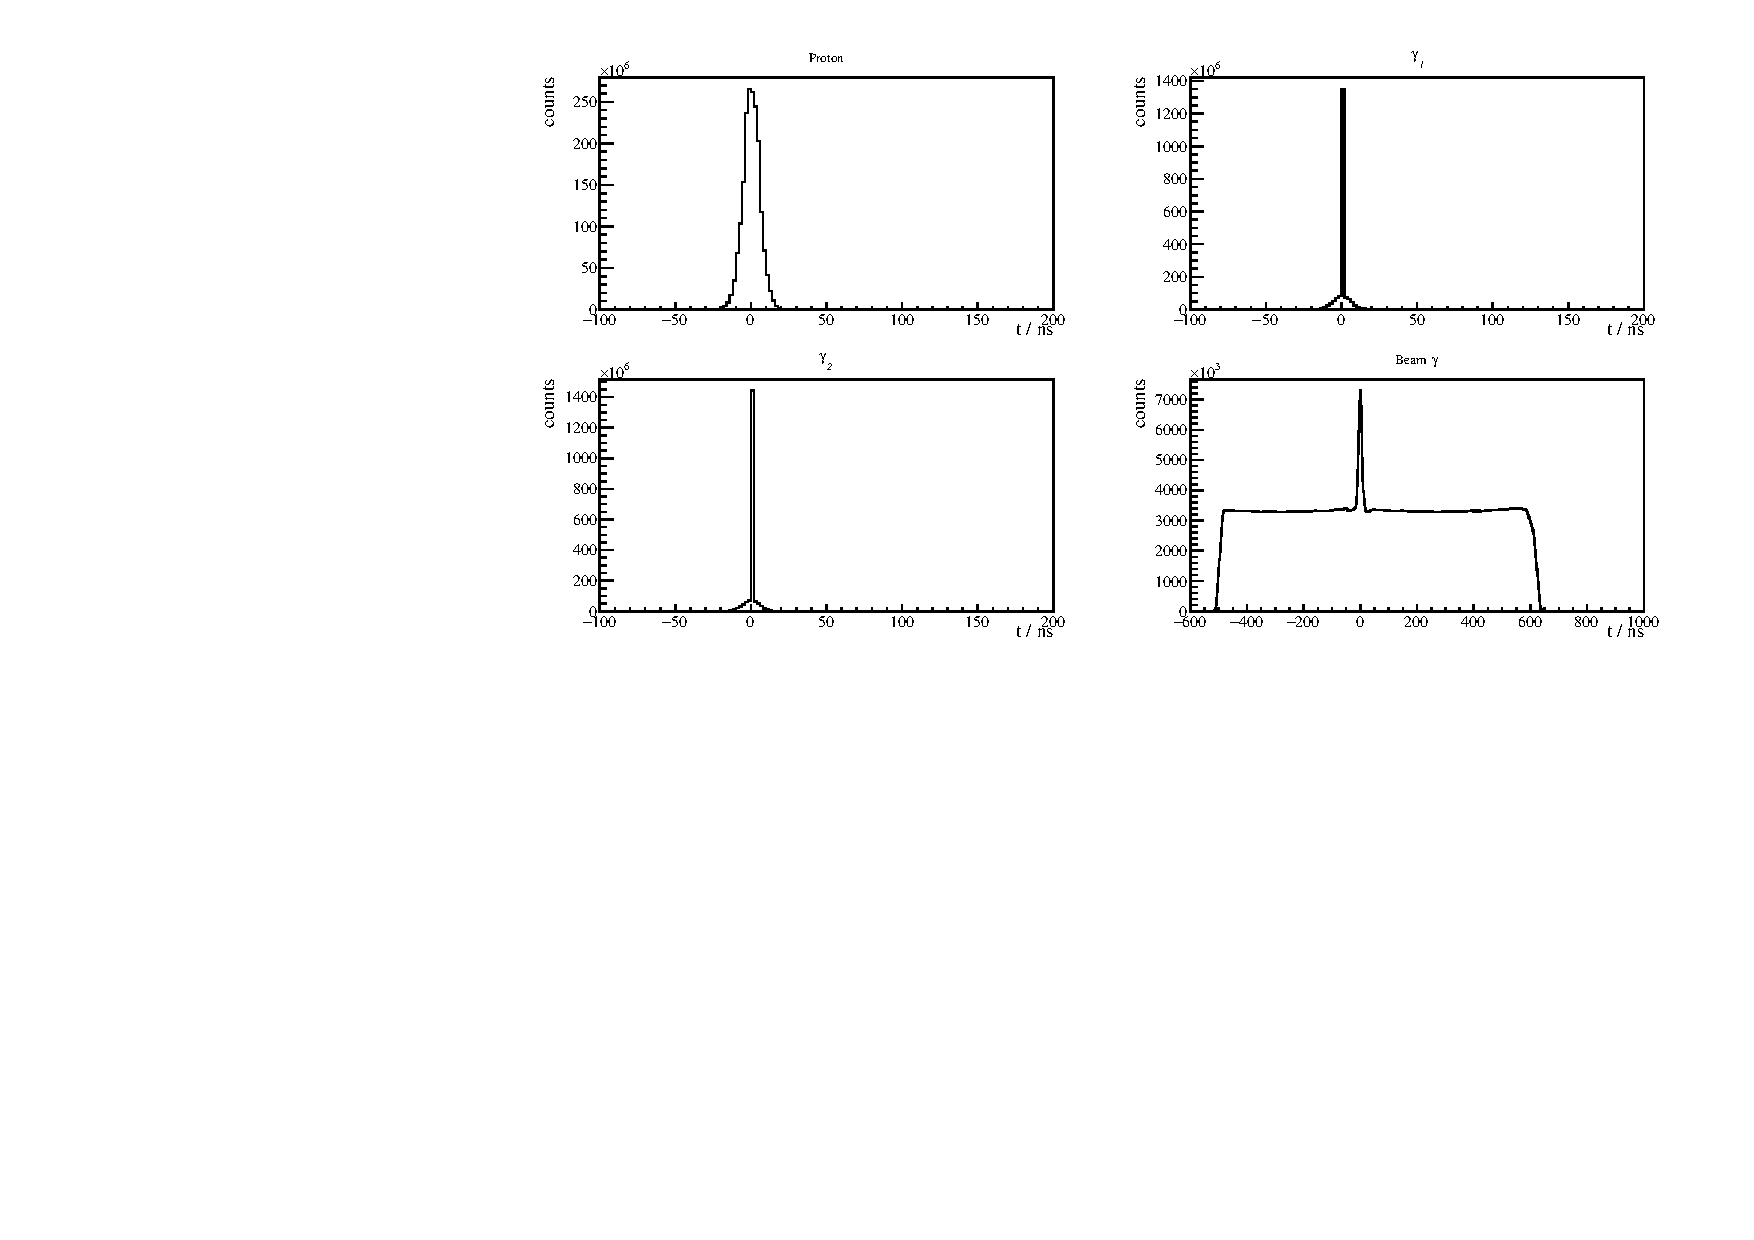
\includegraphics[width=\linewidth]{../figs/hydrogen/time/times.pdf}
	\caption{Time information of all final state particles and the beam photon for 3PED $\eta'$ production}
	\label{fig:time}
\end{figure} 

\begin{figure}[htbp]
	\centering
	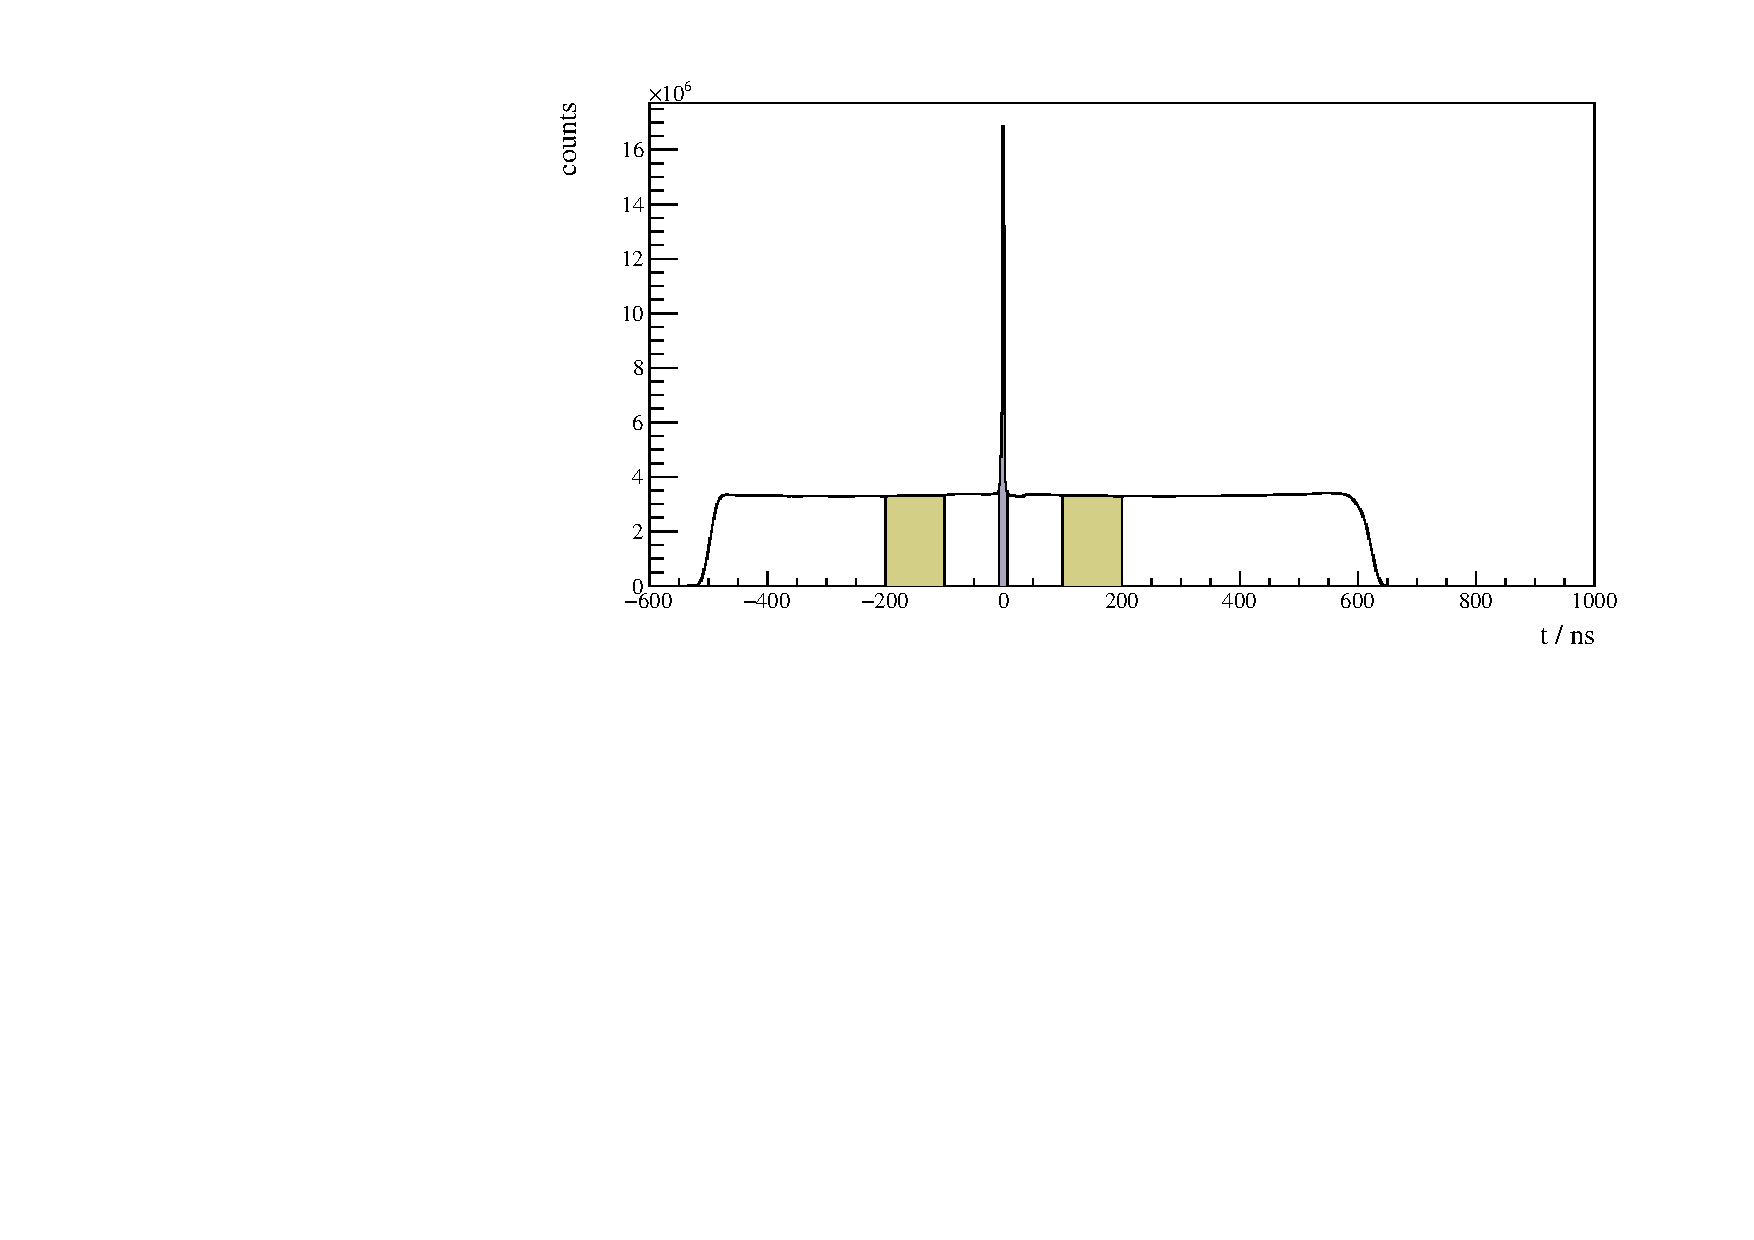
\includegraphics[width=\linewidth]{../figs/hydrogen/time/reaction_time.pdf}
	\caption{Reaction time $t_r$ for 3PED $\eta'$ production}
	\label{fig:time_r}
\end{figure} 